%\title{LaTeX Portrait Poster Template}
%%%%%%%%%%%%%%%%%%%%%%%%%%%%%%%%%%%%%%%%%
% a0poster Portrait Poster
% LaTeX Template
% Version 1.0 (22/06/13)
%
% The a0poster class was created by:
% Gerlinde Kettl and Matthias Weiser (tex@kettl.de)
%
% Adapter by Jens Buysse for Hogeschool Gent
% This template has been downloaded from:
% http://www.LaTeXTemplates.com
%
% License:
% CC BY-NC-SA 3.0 (http://creativecommons.org/licenses/by-nc-sa/3.0/)
%
%%%%%%%%%%%%%%%%%%%%%%%%%%%%%%%%%%%%%%%%%

%----------------------------------------------------------------------------------------
%	PACKAGES AND OTHER DOCUMENT CONFIGURATIONS
%----------------------------------------------------------------------------------------

\documentclass[a0,portrait]{a0poster}

\usepackage{multicol} % This is so we can have multiple columns of text side-by-side
\columnsep=150pt % This is the amount of white space between the columns in the poster
\columnseprule=3pt % This is the thickness of the black line between the columns in the poster

\usepackage[svgnames]{xcolor} % Specify colors by their 'svgnames', for a full list of all colors available see here: http://www.latextemplates.com/svgnames-colors

\usepackage{times} % Use the times font
%\usepackage{palatino} % Uncomment to use the Palatino font

\usepackage{graphicx} % Required for including images
\graphicspath{{figures/}} % Location of the graphics files
\usepackage{booktabs} % Top and bottom rules for table
\usepackage[font=small,labelfont=bf]{caption} % Required for specifying captions to tables and figures
\usepackage{amsfonts, amsmath, amsthm, amssymb} % For math fonts, symbols and environments
\usepackage{wrapfig} % Allows wrapping text around tables and figures
\usepackage[export]{adjustbox}

\begin{document}

%----------------------------------------------------------------------------------------
%	POSTER HEADER
%----------------------------------------------------------------------------------------

% The header is divided into two boxes:
% The first is 75% wide and houses the title, subtitle, names, university/organization and contact information
% The second is 25% wide and houses a logo for your university/organization or a photo of you
% The widths of these boxes can be easily edited to accommodate your content as you see fit

\begin{minipage}[t]{0.75\linewidth}
\VeryHuge \color{HoGentAccent1} \textbf{Nursery Tone Monitor: detecteren van \newline elderspeak via AI} \color{Black}\\ % Title
\Huge\textit{Webapplicatie om elderspeak te detecteren}\\[2.4cm] % Subtitle
\huge \textbf{De Gussem Sibian, Campens Jorrit, Van Boven Geert}\\[0.5cm] % Author(s)
\huge Hogeschool Gent, Valentin Vaerwyckweg 1, 9000 Gent\\[0.4cm] % University/organization
\Large \texttt{sibian.degussem@student.hogent.be} \\
\end{minipage}
%
\begin{minipage}[t]{0.30\linewidth}

\includegraphics[width=13cm,right]{figures/HOGENT_Logo_Pos_rgb.png}

\end{minipage}

\vspace{2cm} % A bit of extra whitespace between the header and poster content

%----------------------------------------------------------------------------------------

\begin{multicols}{2} % This is how many columns your poster will be broken into, a portrait poster is generally split into 2 columns

%----------------------------------------------------------------------------------------
%	ABSTRACT
%----------------------------------------------------------------------------------------

\color{HoGentAccent1} % Navy color for the abstract

\begin{abstract}
Deze bachelorproef is het vervolg op twee eerder gepubliceerde bachelorproefonderzoeken van Beeckman (2021) en Standaert (2021) en zal op een softwarematige manier nagaan of er in een stukje audio \textit{elderspeak} te onderscheiden valt. Een webapplicatie zal aanduiden of er verkleinwoorden of troetelnamen aanwezig waren, of er veel herhaald werd en of de toonhoogte hoger is dan anders. Ook zal er aangeduid worden of er verhoogd stemvolume aanwezig was. Dit zal gerealiseerd worden met Python, spraakherkenning, herkenningsmethoden, \textit{machine learning} of \textit{deep learning} en gepresenteerd worden via een webapplicatie met ``Flask'' als back-end.
\end{abstract}
\vspace{1cm}
%----------------------------------------------------------------------------------------
%	INTRODUCTION
%----------------------------------------------------------------------------------------

\color{HoGentAccent1}
\section*{Introductie}
\color{black}
\color{black}
Deze bachelorproef behandelt het detecteren van \textit{elderspeak} a.d.h.v.\ een webapplicatie. Elderspeak is het fenomeen waarbij jongere mensen tegen ouderen spreken op een betuttelende manier, vandaar dat \textit{elderspeak} ook wel als \textit{secondary baby talk} wordt benoemd.

\newline
Eigenschappen van \textit{elderspeak} zijn: langzaam spreken, verhoogde toonhoogte, verhoogd stemvolume, overdreven intonatie, vereenvoudigd woordgebruik, gebruik van collectieve voornaamwoorden, veelvuldig gebruik van tussenwerpsels, gewijzigd non-verbaal gedrag en veelvuldige verduidelijking en herhalingen. Dit kan voorkomen worden door de volgende tips: vraag of je de voornaam mag gebruiken in een conversatie, vermijd troetelnamen, wees bewust van je non-verbaal gedrag, verhoog het stemvolume enkel wanneer de gesprekspartner hardhorig is, herhalingen en verminderde grammaticale complexiteit kunnen als de andere het niet begrepen heeft, vermijd korte, langzame en overdreven intonatie, vermijd gebruik van verkleinwoorden en hanteer beleefd taalgebruik.


Waarom moet \textit{elderspeak} kunnen gedetecteerd worden? \textit{elderspeak} heeft negatieve gevolgen op de ouderen hun mentale gezondheid. Zo krijgen ze het gevoel dat ze hulpeloos en afhankelijk zijn, het bedreigt hun zelfbeeld, zelfrespect en welzijn. Dit kan bovendien depressieve gevoelens opwerken die zowel fysiek als cognitieve achteruitgang in de hand kunnen werken. Hierdoor zullen sommige ouderen sociale interactie vermijden en mogelijk sociaal geïsoleerd geraken. Het is dus belangrijk dat \textit{elderspeak} vermeden wordt, want het ervaren van sociale betrokkenheid gaat gepaard met een toename van de tevredenheid over het leven.

%----------------------------------------------------------------------------------------
%	GEOLOGY
%----------------------------------------------------------------------------------------

\color{Black} % DarkSlateGray color for the rest of the content
\color{HoGentAccent1}
\section*{Proof-of-concept}
\color{black}

Er werd een basisapplicatie gemaakt die eerst vraagt om te praten zoals je zou doen tegen je vrienden. Nadien wordt er gevraagd om te praten zoals je zou doen bij slechthorende ouderen. Ter ondersteuning zal er een foto getoond worden van iemand uit een woon-zorgcentrum. De applicatie analyseert dan de audiosamples en geeft aan welke kenmerken er aanwezig waren van \textit{elderspeak}. Die kenmerken en de reden waarom het model oordeelt dat die aanwezig zijn, zijn vergaard in het literatuuronderzoek.

In die webapplicatie werd er spraakherkenning die \textit{natural language processing} en artificiële intelligentie gebruiken, gebruikt en het achtergrondlawaai werd ook weggefilterd. Hoe die dat werkt in die Python-bibliotheken.

Om de werking, specificiteit en de sensibiliteit van de applicatie te objectiveren, zijn er
automatische testen opgezet in Python.



%------------------------------------------------



\color{HoGentAccent1}
\section*{Resultaten}
\color{black}

A.d.h.v.\ de \textit{confusion matrices} uit de bachelorproef kan geconcludeerd worden dat er te weinig samples zijn om een beeld te vormen over de effectieve werking van de applicatie. Er moeten meer gevallen verzameld worden waarbij de toonhoogte of het stemvolume hoger is en waarbij er verkleinwoorden aanwezig zijn.

De \textit{requirements} die opgesteld werden zijn wel degelijk voldaan. Zo kan de applicatie de \textit{elderspeak} detecteren, weliswaar met een foutmarge die te lezen is in de bachelorproef zelf. Daarnaast kan de webapplicatie geïnstalleerd worden op een computer en heeft alles een een mooie lay-out gekregen.

Een live-demo van de applicatie kan gevonden worden via de QR-code. In die video op Vimeo wordt gedemonstreerd hoe de applicatie werkt en er uit ziet.

\color{HoGentAccent1}
\section*{Sectie met figuren}
\color{black}

\begin{center}\vspace{1cm}
    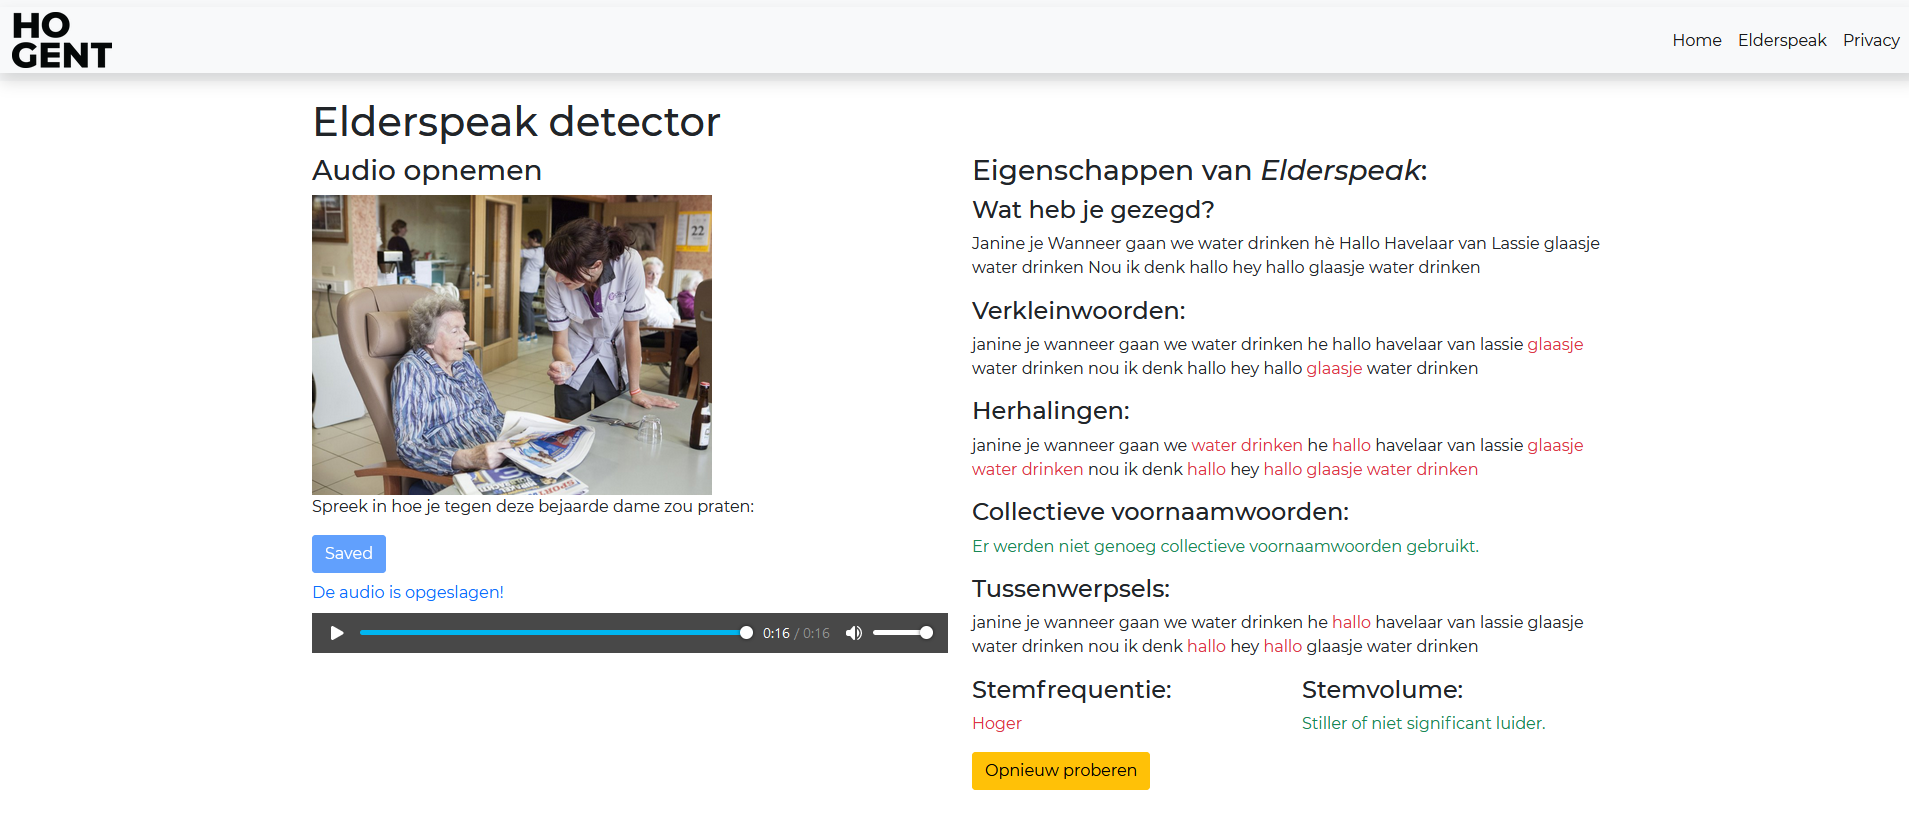
\includegraphics[width=1.0\linewidth]{dector_na_detecteren}
    \captionof{figure}{\color{HoGentAccent5} Screenshot van de webapplicatie na het analyseren van een audiofragment.}
\end{center}\vspace{1cm}

\begin{center}\vspace{1cm}
    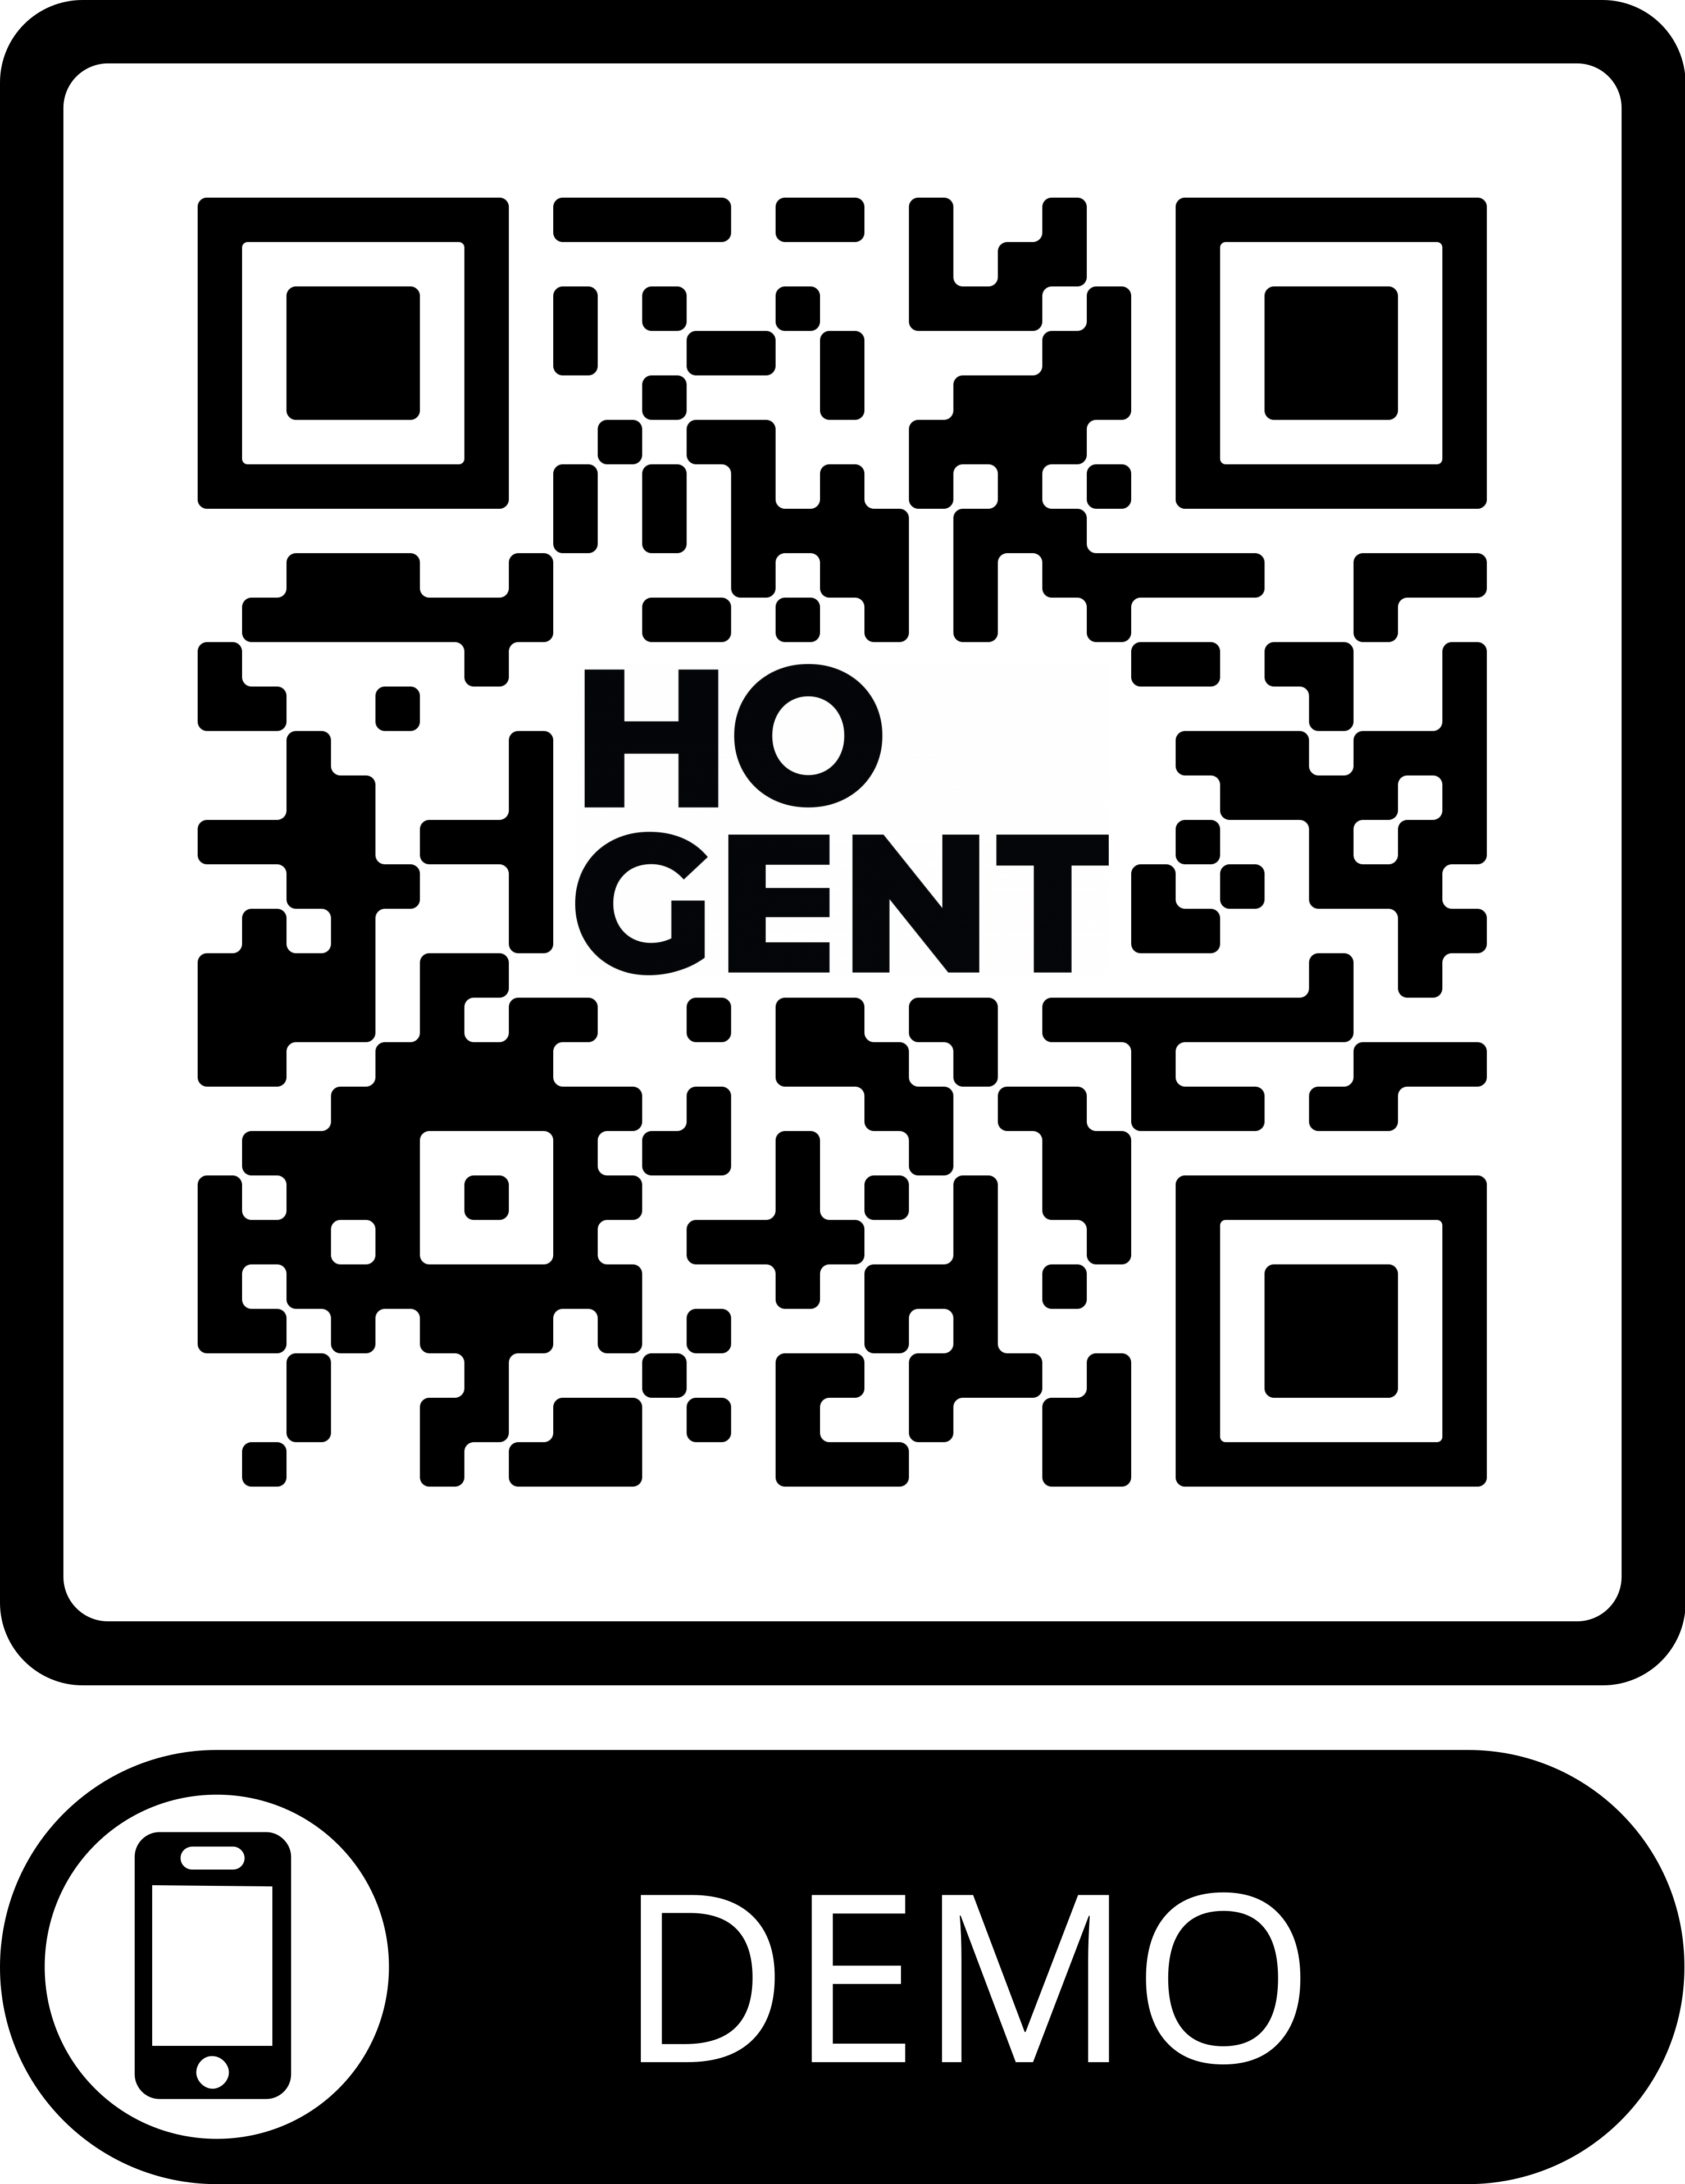
\includegraphics[width=0.25\linewidth]{qr}
    \captionof{figure}{\color{HoGentAccent5} Scan de QR-code om een live demo te zien.}
\end{center}\vspace{1cm}


%----------------------------------------------------------------------------------------
%	FORTHCOMING RESEARCH
%----------------------------------------------------------------------------------------
\color{HoGentAccent1}
\section*{Toekomstig onderzoek}
\color{black}

Het aantal testen dat verzameld werd, is niet van een bijzonder grote grootteorde. Er kunnen extra testen, in de vorm van nieuwe audio-opnames, opgenomen worden in een vervolgopdracht. Dit kan een interdisciplinaire opdracht zijn met de richting verpleegkunde, communicatie en eventueel toegepaste informatica. Immers hoe meer testen, hoe groter de accuraatheid van de applicatie. Studenten uit communicatierichtingen kunnen alle data dan opnieuw labelen, aangezien zij veel kennis hebben rond dit fenomeen. Zo kan de data zeer nauwkeurig en uitgebreid geanalyseerd worden, terwijl in dit eindwerk de data gelabeld werd door een persoon die geen expert is.

%----------------------------------------------------------------------------------------


%----------------------------------------------------------------------------------------
%	Usage
%----------------------------------------------------------------------------------------
\color{HoGentAccent1}
\section*{Gebruik van de applicatie}
\color{black}

Concluderend kunnen we stellen dat deze applicatie zeker en vast gebruikt kan worden voor studenten in de zorgsector. Op die manier kunnen ze \textit{elderspeak} ontdekken en het fenomeen beter leren herkennen. Dat kan zowel actief, via de detector, als passief, door de lijst van eigenschappen en tips te lezen.

De accuraatheid is niet ideaal, maar dat hoeft ook niet. Wanneer iemand de detector gebruikt, is het belangrijk dat hij of zij ook aan zelfreflectie doet. Op die manier blijven het begrip en de eigenschappen langer aanwezig in het geheugen.

%----------------------------------------------------------------------------------------

\end{multicols}
\end{document}